\documentclass[12pt,a4paper]{article}

% ============================================================
% PACKAGES
% ============================================================
\usepackage[
    a4paper,
    top=1.55cm,
    bottom=1.35cm,
    left=1.75cm,
    right=1.75cm
]{geometry}
\usepackage{enumitem}
\usepackage[T1]{fontenc}
\usepackage{newtxtext}
\usepackage{graphicx}
\usepackage{xcolor}
\usepackage{array}
\usepackage{tabularx}
\usepackage{fancyhdr}
\usepackage{tikz}
\usepackage{eso-pic}
\usepackage{ragged2e}

% ============================================================
% COLORS
% ============================================================
\definecolor{GEUBlue}{RGB}{43,91,145}
\definecolor{GEUBannerBlue}{RGB}{0,102,148}
\definecolor{GEUYellow}{RGB}{255,201,38}
\definecolor{InstructionGrey}{RGB}{125,125,125}

% ============================================================
% GENERAL SETTINGS
% ============================================================
\setlength{\parindent}{0pt}
\setlength{\parskip}{0pt}
\renewcommand{\arraystretch}{1}

% ============================================================
% HEADER / FOOTER
% ============================================================
\pagestyle{fancy}
\fancyhf{}

\fancyhead[L]{%
    \fontsize{10.5}{12}\selectfont
    B.TECH (CSE) - DSCPP-III-2026-T078
}

\fancyhead[R]{%
    \fontsize{10.5}{12}\selectfont
    PHASE-III PROJECT PROGRESS
}

\fancyfoot[R]{%
    \fontsize{10}{12}\selectfont
    Page \thepage
}

\renewcommand{\headrulewidth}{0pt}
\renewcommand{\footrulewidth}{0pt}

\setlength{\headheight}{20pt}
\setlength{\headsep}{0.65cm}
\setlength{\footskip}{0.65cm}

% ============================================================
% BOTTOM YELLOW LINE
% ============================================================
\AddToShipoutPictureBG{%
\begin{tikzpicture}[remember picture,overlay]
    \fill[GEUYellow]
    (current page.south west)
    rectangle
    ([yshift=0.14cm]current page.south east);
\end{tikzpicture}
}

% ============================================================
% CUSTOM COMMANDS
% ============================================================
\newcommand{\sectiontitle}[1]{%
    {\color{GEUBlue}
    \fontsize{18}{22}\selectfont #1}
}

\newcommand{\instruction}[1]{%
    {\color{InstructionGrey}
    \fontsize{10.5}{13}\selectfont #1}
}

\newcommand{\answerbox}[2]{%
    \begin{tabularx}{\textwidth}{
        |>{\raggedright\arraybackslash}X|}
        \hline
        \parbox[t][#1][t]{\dimexpr\linewidth-12pt\relax}{
            \vspace{5pt}
            \fontsize{11}{13}\selectfont #2
        }\\
        \hline
    \end{tabularx}
}

% ============================================================
% DOCUMENT
% ============================================================
\begin{document}

% ============================================================
% PAGE 1
% ============================================================

\vspace*{0.10cm}

\includegraphics[width=8.0cm]{geulogo.png}

\vspace{0.70cm}

\noindent
\colorbox{GEUBannerBlue}{%
\parbox{\dimexpr\textwidth-2\fboxsep\relax}{
    \vspace{0.17cm}
    {\color{GEUYellow}
    \fontsize{16.5}{20}\selectfont
    \bfseries
    PROJECT AND TEAM INFORMATION}
    \vspace{0.17cm}
}}

\vspace{0.80cm}

% PROJECT TITLE
\sectiontitle{Project Title}

% \vspace{0.05cm}

% \instruction{(Try to choose a catchy title. Max 20 words).}

\vspace{0.40cm}

\answerbox{1.00cm}{TapNGo - A Bus Fare Verification And Payment System}

\vspace{0.80cm}

% TEAM INFORMATION
% \sectiontitle{Student/Team Information}

% \vspace{0.40cm}

% \begin{tabularx}{\textwidth}{
% |>{\raggedright\arraybackslash}p{0.66\textwidth}
% |>{\raggedright\arraybackslash}X|
% }
% \hline

% \parbox[t][1.15cm][t]{\linewidth}{
% \vspace{4pt}
% \fontsize{10.5}{13}\selectfont
% Team Name:\\[2pt]
% Team \# (Mentor needs to assign)
% }
% &
% \\
% \hline

% \parbox[t][3.65cm][t]{\linewidth}{
% \vspace{5pt}
% \fontsize{10.5}{13}\selectfont
% Team member 1 (Team Lead)\\[3pt]
% {\color{InstructionGrey}
% (Last Name, name: student ID: email, picture):}
% }
% &
% \\
% \hline

% \parbox[t][3.65cm][t]{\linewidth}{
% \vspace{5pt}
% \fontsize{10.5}{13}\selectfont
% Team member 2\\[3pt]
% {\color{InstructionGrey}
% (Last Name, name: student ID: email, picture):}
% }
% &
% \\
% \hline

% \end{tabularx}

% \newpage

% ============================================================
% PAGE 2
% ============================================================
\noindent
\begin{tabularx}{\textwidth}{|>{\RaggedRight\arraybackslash}p{0.69\textwidth}|>{\RaggedRight\arraybackslash}X|}
\hline
\begin{minipage}[t]{\linewidth}
\vspace{1.5mm}
\textit{Team Name:}\\[-1mm]
\textit{Team \#}
\vspace{1.5mm}
\end{minipage}
&
\begin{minipage}[t]{\linewidth}
\vspace{1.5mm}
\textit{A3K}\\
\textit{DSCPP-III-2026-T078}
\vspace{1.5mm}
\end{minipage}
\\
\hline
\begin{minipage}[t][3.25cm][t]{\linewidth}
\vspace{1.5mm}
\textbf{Team member 1 (Team Lead)}\\[-1mm]
\textit{(Last Name, name: student ID: email, picture):}
\vspace{2.0cm}
\end{minipage}
&
\begin{minipage}[t][3.25cm][t]{\linewidth}
\vspace{1.5mm}
\textit{Jain, Karnika -- 2510010541}\\
\textit{karnikajain90@gmail.com}

\vspace{2mm}
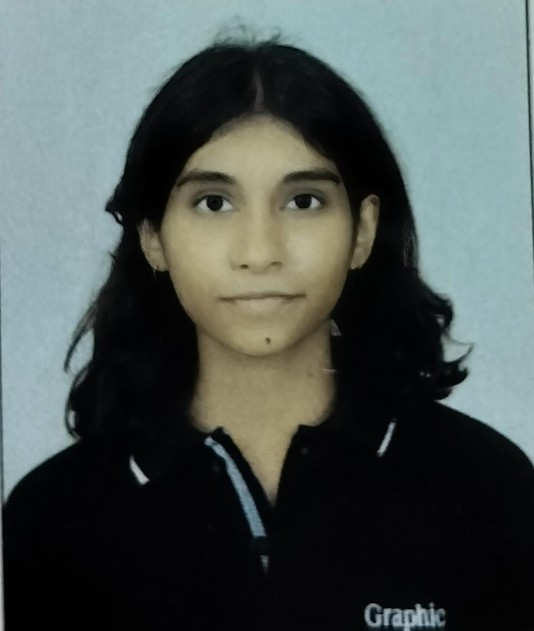
\includegraphics[width=3.0cm,height=1.5cm,keepaspectratio]{member1.png}
\end{minipage}
\\
\hline
\begin{minipage}[t][3.25cm][t]{\linewidth}
\vspace{1.5mm}
\textbf{Team member 2}\\[-1mm]
\textit{(Last Name, name: student ID: email, picture):}
\vspace{2.0cm}
\end{minipage}
&
\begin{minipage}[t][3.25cm][t]{\linewidth}
\vspace{1.5mm}
\textit{Bahuguna, Anirudh -- 2510013536}\\
\textit{anirudhbahuguna14@gmail.com}

\vspace{2mm}
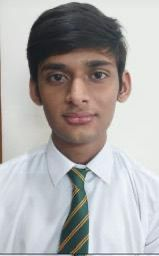
\includegraphics[width=3.0cm,height=1.5cm,keepaspectratio]{member2.png}
\end{minipage}
\\
\hline
\begin{minipage}[t][3.25cm][t]{\linewidth}
\vspace{1.5mm}
\textbf{Team member 3}\\[-1mm]
\textit{(Last Name, name: student ID: email, picture):}
\vspace{2.0cm}
\end{minipage}
&
\begin{minipage}[t][3.25cm][t]{\linewidth}
\vspace{1.5mm}
\textit{Budakoti, Aaditya -- 2510290931}\\
\textit{aadityabudakoti@gmail.com}

\vspace{2mm}
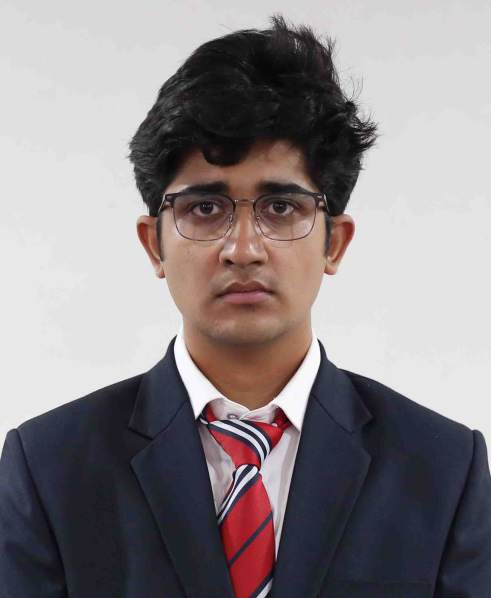
\includegraphics[width=3.0cm,height=1.5cm,keepaspectratio]{member3.png}
\end{minipage}
\\
\hline
\begin{minipage}[t][3.25cm][t]{\linewidth}
\vspace{1.5mm}
\textbf{Team member 4}\\[-1mm]
\textit{(Last Name, name: student ID: email, picture):}
\vspace{2.0cm}
\end{minipage}
&
\begin{minipage}[t][3.25cm][t]{\linewidth}
\vspace{1.5mm}
\textit{Pant, Aparajita -- 2510011139}\\
\textit{aparajitapant246@gmail.com}

\vspace{2mm}
 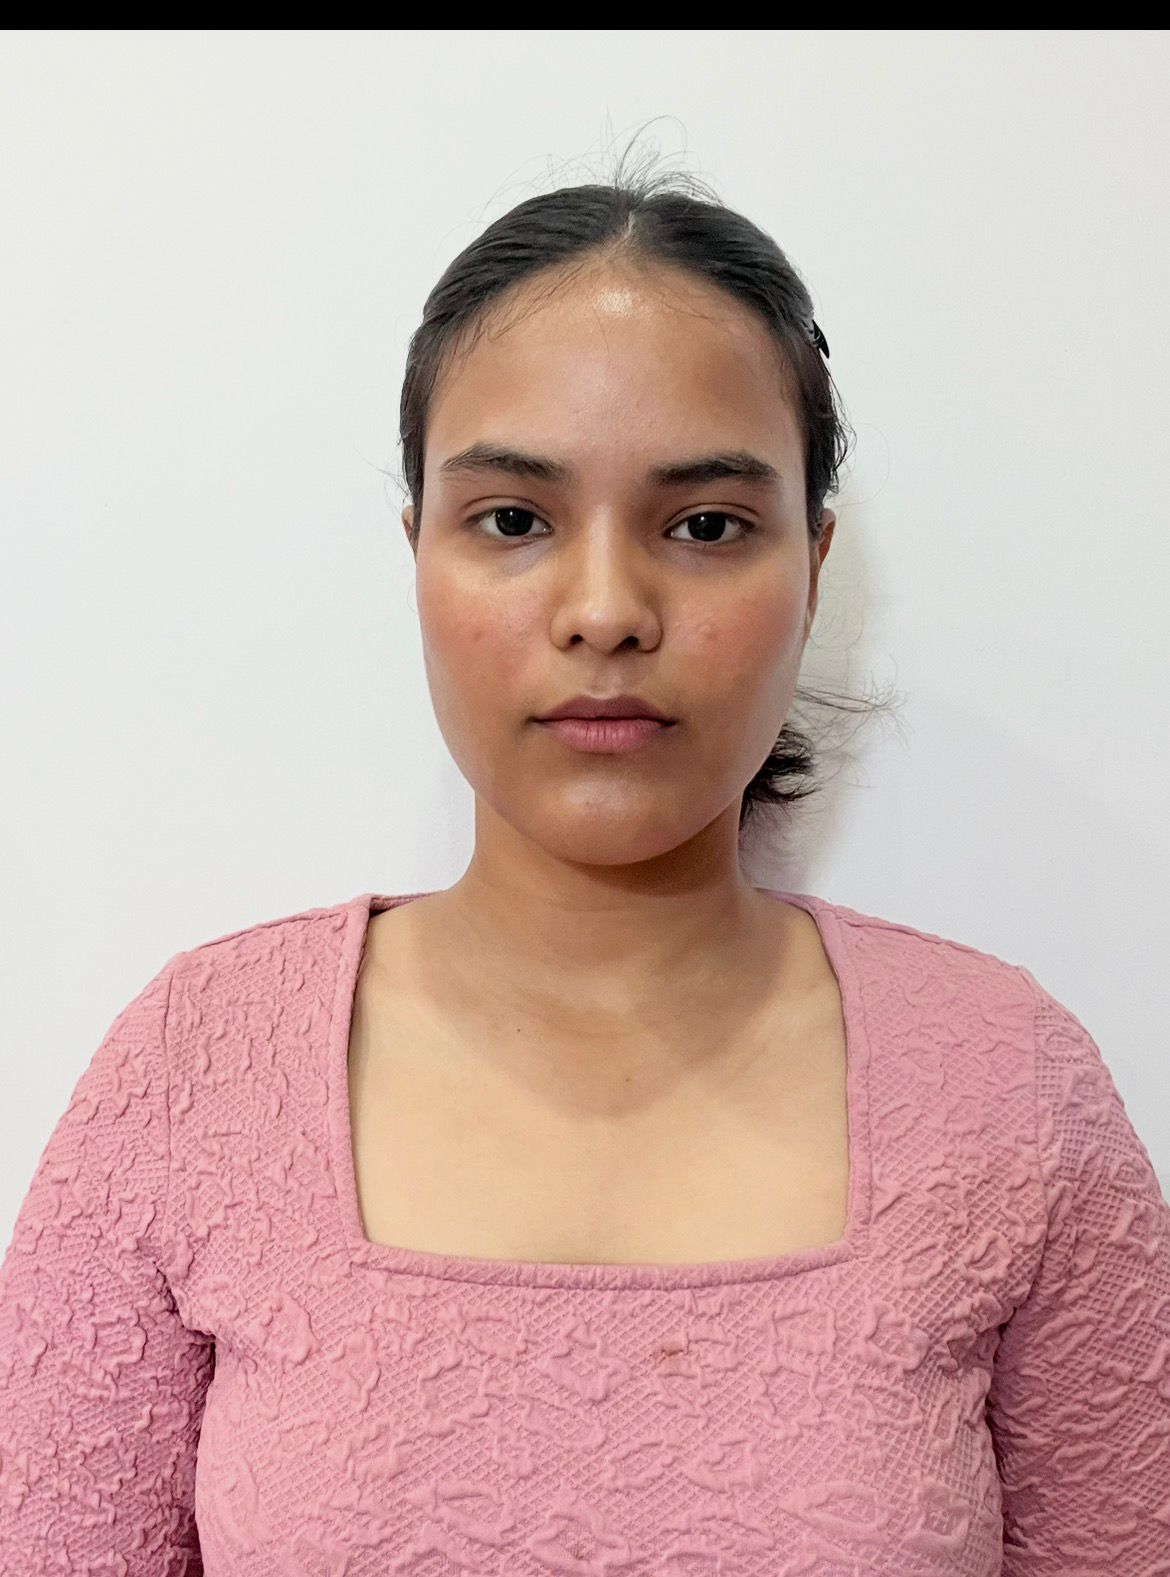
\includegraphics[width=3.0cm,height=1.5cm,keepaspectratio]{member4.png}
\end{minipage}
\\
\hline
\end{tabularx}

\newpage
\vspace*{0.15cm}

\noindent
\colorbox{GEUBannerBlue}{%
\parbox{\dimexpr\textwidth-2\fboxsep\relax}{
    \vspace{0.18cm}
    {\color{GEUYellow}
    \fontsize{17}{21}\selectfont
    \bfseries
    PHASE-III PROJECT PROGRESS DESCRIPTION (35 pts)}
    \vspace{0.18cm}
}}

\vspace{0.70cm}

% ABSTRACT
\sectiontitle{Project Abstract (2 pts)}

\vspace{0.05cm}

% \instruction{
% (Brief restatement of your project's main goal. Max 300 words).
% }

% \vspace{0.12cm}

\answerbox{6cm}{Our project TapNGo is an automated bus fare verification and seat monitoring system which is designed to help reduce boarding delays due to manual fare verification processes. It aims to reduce the time taken and the human error in verifying each seat's payment by the use of a digital verification process. Thus saving time and effort and also reducing the room for errors.\\

It does so by categorizing each seat in the bus into 3 categories:\\
1. Empty\\
2. Occupied and Unverified\\
3. Occupied and Verified\\

Once the driver/conductor is satisfied with the seating and payment verification of all the passengers, they can depart to the next station. }

\vspace{0.70cm}

% UPDATED APPROACH
\sectiontitle{Updated Project Approach and Architecture (2 pts)}

% \vspace{0.05cm}

% \instruction{
% (Describe your current approach, including system design,
% communication protocols, libraries used, etc.\\
% Max 300 words).
% }

\vspace{0.25cm}

\answerbox{15cm}{The Approach we have gone with to make this project is by dividing the entire things into 3 parts that follows the System Design given below:\\
\vspace{2mm}
\begin{center}
    \includegraphics[width=25cm,height=8cm,keepaspectratio]{System_Arch_PIII.png}
\end{center}
\vspace{2mm}\\
Tech Stack:\\
Programming Language : C++ 17\\
Standard Libraries   : C++ STL\\
IDE                  : VS Code\\
Version Control      : Git and GitHub\\

We have focused on creating a software only PBL prototype that works entirely by going through different modules. All this has being designed to run on a single system thus eliminating the requirement for a network/communication protocol
}

\newpage

% ============================================================
% PAGE 3
% ============================================================

\vspace*{0.20cm}

% TASKS COMPLETED
\sectiontitle{Tasks Completed (7 pts)}

\vspace{0.05cm}


\vspace{0.20cm}

\begin{tabularx}{\textwidth}{
|>{\raggedright\arraybackslash}X
|>{\raggedright\arraybackslash}X|
}
\hline

\textbf{Task Completed} &
\textbf{Team Member}
\\[0.3cm]
\hline

\parbox[t][4.5cm][t]{\linewidth}{Integrated all seat management modules \& tested overall system capability.\\[0.1cm]
Integrated and tested fare verification logic, valid \& invalid card verification situations.\\[0.1cm]
Performed system testing, data validation, edge cases, \& debugging .\\[0.1cm]
Integrated departure readiness logic, finalized the driver panel, \& prepared final documentation.}
&
\parbox[t][4.5cm][t]{\linewidth}{Karnika Jain\\[0.7cm]
Anirudh Bahuguna\\[0.7cm]
Aaditya Budakoti\\[0.7cm]
Aparajita Pant}
\\
\hline

\end{tabularx}

\vspace{0.65cm}

% CHALLENGES
\sectiontitle{Challenges/Roadblocks (7 pts)}

\vspace{0.05cm}


\vspace{0.18cm}

\answerbox{5.05cm}{During Phase III, the major challenges we faced were integrating the C++ modules that were developed independently and ensuring coordination between different classes and functions.Another challenge we faced  was maintaining accurate seat state logic while occupancy detection and fare verifications. Handling  edge cases like invalid cards taps and logic and runtime errors during testing was also an problem we faced. \\[0.2cm] The problems were  fixed through the debug process and by running many tests cases. Module integration problems were solved by checking the interfaces of classes ,functions and ensuring they are all working together. Logic for seat statuses was made better by verifying them and once they were detected as occupied and price checked. Invalid cards taps were fixed by displaying the correct message and improving verification proccess. Runtime and logic errors were found by running many tests. }

\vspace{0.65cm}

% TASKS PENDING
% \sectiontitle{Tasks Pending (7 pts)}

% \vspace{0.05cm}

% \instruction{
% (Describe the main tasks that you still need to complete.
% Max 250 words).
% }

% \vspace{0.18cm}

% \begin{tabularx}{\textwidth}{
% |>{\raggedright\arraybackslash}X
% |>{\raggedright\arraybackslash}X|
% }
% \hline

% \textbf{Task Pending} &
% \textbf{Team Member (to complete the task)}
% \\
% \hline

% \parbox[t][1.25cm][t]{\linewidth}{}
% &
% \parbox[t][1.25cm][t]{\linewidth}{}
% \\
% \hline

% \end{tabularx}

% \newpage

% ============================================================
% PAGE 4
% ============================================================

\vspace*{0.30cm}


% OUTCOMES
\sectiontitle{Project Outcome/Deliverables (2 pts)}

\vspace{0.35cm}

\answerbox{6.6cm}{At the end of Phase III, we have a working C++17 console program that checks fares seat by seat, so the conductor doesn’t have to check everyone at the door. This is what we are submitting:\\[-0.6cm]
\begin{itemize}[leftmargin=7pt]
\setlength{\itemsep}{0pt}
\setlength{\parskip}{0pt}
\setlength{\topsep}{0pt}
\item Seat tracking: each seat shows as Empty, Occupied–Unverified or Occupied–Verified, and it is updated as passengers get on, pay or get off.\\[-0.4cm]
\item Fare chart: fares for our 12-stop Dehradun route (ISBT to Rajpur), stored in a 12 × 12 matrix so the fare between any two stops can be looked up.\\[-0.4cm]
\item Simulated card tap: it checks that the card number is valid and then marks that seat as paid.\\[-0.4cm]
\item Transaction queue: a linked list that records each payment and removes it once the passenger leaves.\\[-0.4cm]
\item Driver dashboard: it shows seats in grey, red or green depending upon the seat status ,and won’t let the bus leave if anyone on the bus hasn’t paid for their seat yet.\\[-0.6cm]
\end{itemize}
Along with the program we have a test file with 28 checks, the README, an architecture document and our phase reports.}

% PROGRESS
\newpage

\sectiontitle{Progress Overview (2 pts)}

\vspace{0.05cm}

\instruction{
(Summarize how much of the project is done, what's behind schedule,
what's ahead of schedule. Max 200 words.)
}

\vspace{0.25cm}

\answerbox{6.3cm}{Everything we planned for the software prototype is now done. The Bus, Passenger and Payment classes are written and connected through \texttt{main.cpp}, so a full run works: a passenger takes a seat, pays, shows up on the dashboard, and once everyone has paid the bus is cleared to leave. All 28 checks in our test file pass.

A couple of things went further than we first planned. Earlier we were using a flat rate per km, but we replaced that with a proper stop-to-stop fare chart for 12 real stops in Dehradun, and the driver dashboard now uses colours so unpaid seats are easy to spot.

We fell behind around 25 October. Our code was split across eight folders and connecting it was getting messy, so we merged it into three main classes. That set us back by roughly a week. We also dropped the separate database module and kept the data in arrays, vectors and a linked-list queue instead. Real card readers or NFC are left as future work.}

\vspace*{0.20cm}

% CODEBASE
\sectiontitle{Codebase Information (2 pts)}

\vspace{0.05cm}

\instruction{
(Repository link, branch, and information about important commits.)
}

\vspace{0.20cm}

\answerbox{7.2cm}{\textbf{Repository:} https://github.com/kjj2608/TapNGo

\textbf{Branch:} We work on \texttt{main}. The fare chart was built on a separate branch, \texttt{stop-selection}, and merged in through Pull Request \#1.

\textbf{How it's organised:} header files are in \texttt{include/}, the class code is in \texttt{src/}, the menu program is \texttt{main.cpp}, tests are in \texttt{test/test.cpp}, and our reports and slides are in \texttt{Documentation/}.

\textbf{Commits worth noting:}
\begin{itemize}\setlength{\itemsep}{0pt}\setlength{\parskip}{0pt}\setlength{\topsep}{2pt}
\item \texttt{ed42619} (16 Oct) -- put the test cases from every branch in one place.
\item \texttt{3950336}, \texttt{fee2e97} (17 Oct) -- edge-case tests and \texttt{architecture.md}.
\item \texttt{4da6414}, \texttt{e235149} (20 Oct) -- cleaned up the TransactionQueue and the departure condition.
\item \texttt{c650f5f}, \texttt{d5e5b7c}, \texttt{042b4c7} (25 Oct) -- rewrote the code as the Bus, Passenger and Payment classes.
\item \texttt{474e19d}, \texttt{958ab84} (3 Nov) -- added the fare chart, route map and removing transactions.
\item \texttt{5c5c2ab} (3 Nov) -- merged Pull Request \#1 (\texttt{stop-selection}).
\end{itemize}}

\newpage

% TESTING
\sectiontitle{Testing and Validation Status (2 pts)}

\vspace{0.05cm}

\instruction{(Provide information about any tests conducted)}

\vspace{0.30cm}

\begin{tabularx}{\textwidth}{
|>{\raggedright\arraybackslash}p{0.30\textwidth}
|>{\raggedright\arraybackslash}p{0.13\textwidth}
|>{\raggedright\arraybackslash}X|
}
\hline
\textbf{Test Type} & \textbf{Status (Pass/Fail)} & \textbf{Notes}\\
\hline
Unit -- Passenger details & Pass & A passenger needs both an ID and a name; if either is missing they are not accepted.\\
\hline
Unit -- Seat states & Pass & Checked the full cycle Empty $\rightarrow$ Unverified $\rightarrow$ Verified $\rightarrow$ Empty. Booking a taken seat or a seat number that doesn't exist fails, as it should.\\
\hline
Unit -- Fare chart & Pass & ISBT to Clock Tower gives Rs 25 and ISBT to Rajpur gives Rs 45. Same start and end stop, or a stop outside 0--11, is refused.\\
\hline
Unit -- Card check & Pass & Card numbers of 4 to 16 digits go through; a 2-digit or 17-digit number is rejected.\\
\hline
Unit -- Transaction queue & Pass & Tried adding and removing from the front, middle and end, removing when the queue is empty, and adding again after it was emptied.\\
\hline
Integration -- Departure check & Pass & The bus is held while any seat is unpaid, and allowed to go once every occupied seat is paid (or the bus is empty).\\
\hline
System -- Full console run & Pass & Went through the whole menu: taking a seat, paying, using a wrong card, leaving a seat, the dashboard and the transaction list.\\
\hline
Memory check (AddressSanitizer) & Pass & No crashes, out-of-range access or memory leaks were reported.\\
\hline
\multicolumn{3}{|l|}{\textbf{Overall:} all 28 checks in \texttt{test/test.cpp} pass.}\\
\hline
\end{tabularx}

\vspace{0.65cm}

% DELIVERABLES
\sectiontitle{Deliverables Progress (2 pts)}

\vspace{0.05cm}

\instruction{
(Summarize the current status of all key project deliverables mentioned earlier. Indicate whether each deliverable is
completed, in progress, or pending.)
}

\vspace{0.25cm}

\answerbox{5.3cm}{\textbf{Seat tracking (Bus class)}: Completed.

\textbf{Passenger class}: Completed.

\textbf{Fare chart and route map (12 stops)}: Completed.

\textbf{Card check and payment}: Completed.

\textbf{Transaction queue}: Completed.

\textbf{Driver dashboard and departure check}: Completed.

\textbf{Menu program (\texttt{main.cpp})}: Completed, builds and runs from start to finish.

\textbf{Test file}: Completed, 28 out of 28 checks pass.

\textbf{Documentation (README, architecture, Phase I--III reports)}: Completed.

\textbf{Card reader / NFC hardware and a database}: Not part of this prototype; kept for future work.}

\end{document}
